%! TEX root = ../main.tex
\documentclass[main]{subfiles}


\begin{document}
\chapter{高速・高信頼センシングシステムの構築}
この章で、ハードウェア/組み込み技術の高さを明確に示す
\section{システム全体の概要}
AGVプラットフォーム(GS02ベース)、搭載センサ群(Mid360, IMU, ZED-F9P, VESC, 生態センサユニット)、ソフトウェア(ROS 2)からなる全体構成を示す(ブロック図)。

TFツリーを示し、特にLiDARの傾斜搭載について言及する。

\section{センサユニットの開発}
本研究で構築するセンサユニットは,植生状態の観察を目的とし,
浜松ホトニクス製ミニ分光器 C12880MA を搭載する.生育環境の評価のため,
Bosch Sensortec 製 BME280(秋月電子通商製ブレークアウト基板 AE-BME280)および 
ELT SENSOR 社製 S300L-3V $CO_2$センサを統合した.
STMicroelectronics製マイクロコントローラ(MCU)を使用し,センサデータを収集する.
本センサユニットの全体構成を Fig.~\ref{fig:agv_multisensor_overall} に示す.
各センサおよびMCUのインタフェース回路を付録に示す
(Fig.~\ref{fig:mcu_circuit},Fig.~\ref{fig:c12880ma_circuit},
Fig.~\ref{fig:s300l_circuit},Fig.~\ref{fig:bme280_circuit}).

\subsection{高速分光センサ駆動モジュールの開発における従来の課題} 
C12880MAセンサは,
入力ST信号立下り後,TRG信号を出力し,
第89番目のTRG(トリガ)信号立上りでVideo信号を出力する.
そのタイミングをFig.~\ref{fig:c12880ma_timing}に示す.

従来は,TRG信号の立ち上がりで割り込みを発生させ,割り込みサービスルーチン(以下,ISR)内で
ADCデータを読み取る割り込み駆動方式を用いてきた.本研究室の先行研究では,
LPC1768 MCUと外部ADコンバータ(SPI接続)を用い,この方式でC12880MAから
\SI{50}{\kilo\hertz}でのデータ取得が報告されている\cite{ref:Kobayashi2021AGV}.
しかしこの方式では,取得ごとにCPUがISRを必ず実行する必要があるため,
割り込み応答遅延が主要な性能制約となり,センサが持つ数\SI{}{\mega\hertz}帯の性能を
引き出すことは困難である.

この制約を再確認するため,内部ADCが高速なSTM32F446REでもISRの方式を検証した.
結果はTable~\ref{tab:previous_method_limit}のとおりであり,
割り込みのみでは\SI{25.4}{\kilo\hertz}付近で欠落が発生した.
さらにDMA(Direct Memory Access;CPUを介さずに周辺装置と
メモリ間でデータを自動転送する仕組み.以下,DMA)を
併用することでCPU負荷は低減し,取得可能周波数は\SI{130}{\kilo\hertz}まで向上したが,
遅延は残存し,数\SI{}{\mega\hertz}帯には到達しなかった.
以上より,割り込み起動時の遅延は問題であることが確認された.

\begin{table}[t]
    \centering
    \caption{Limits of acquisition frequency with conventional methods}
    \label{tab:previous_method_limit}
    \begin{tabular}{l|l|c}
        \hline
        \textbf{Method} & \textbf{MCU} & \textbf{Achieved frequency} \\
        \hline \hline
        Interrupt only      & STM32F446RE & \SI{25.4}{\kilo\hertz}\\
        Interrupt + DMA     & STM32F446RE & \SI{130}{\kilo\hertz} \\
        \hline
    \end{tabular}
\end{table}

\begin{figure}[t]
  \centering
  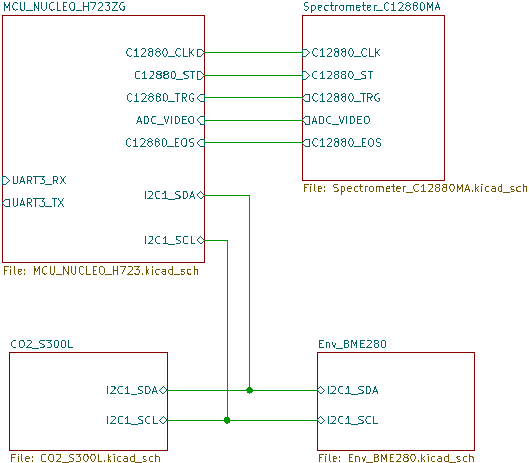
\includegraphics[width=\linewidth]{figures/2/AGV_Multisensor.pdf}
  \caption{Overall multisensor system architecture}
  \label{fig:agv_multisensor_overall}
\end{figure}

% ===== C12880MA Timing Diagram Placeholder =====

\begin{figure}[t]
  \centering
  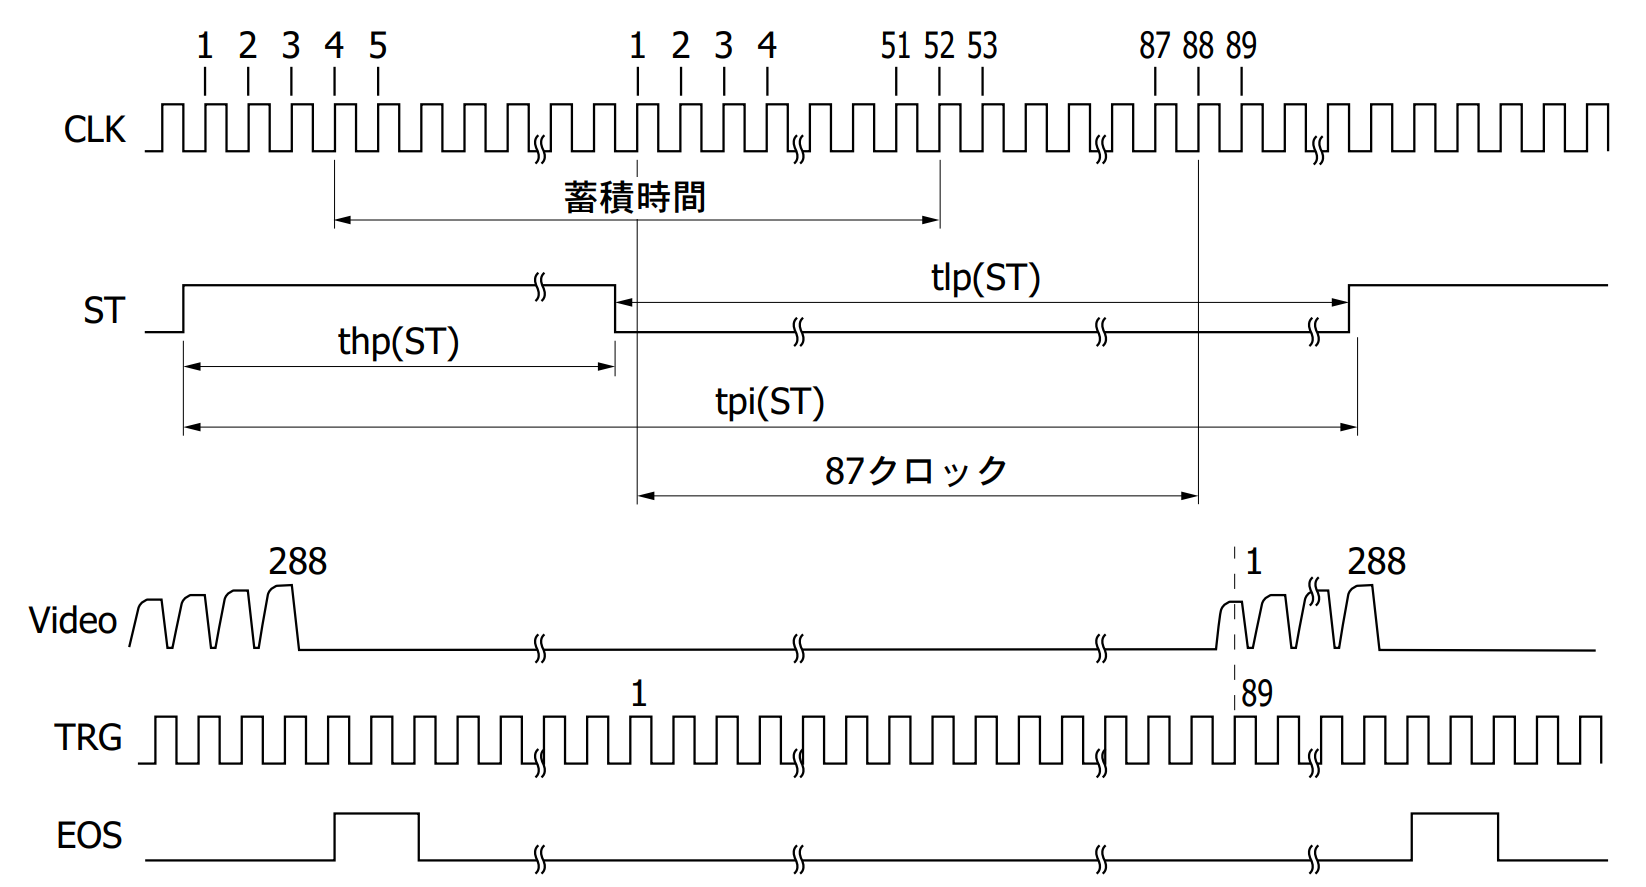
\includegraphics[width=0.9\linewidth]{figures/2/placeholder_C12880MA_timing.png}
  \caption{Timing diagram of the C12880MA: excerpted from the Hamamatsu Photonics datasheet\cite{ref:C12880MA}}
  \label{fig:c12880ma_timing}
\end{figure}




\subsection{提案手法:デュアルスイッチFSMアーキテクチャ}
\label{sec:new_architecture}
割り込み遅延を排除するため,タイマ・ADC・DMAをハードウェアトリガで直結する
アーキテクチャ(Timer$\rightarrow$TRGO$\rightarrow$ADC$\rightarrow$DMA)は必須である.
しかし,この構成にはC12880MA特有の「競合状態(Race Condition)」
の問題が存在する.

\subsubsection{C12880MA駆動における「フライングスタート」問題} 
C12880MAのTRG信号は,CLK(クロック)信号のミラであり,
CLKが供給されている限りTRGも常時出力され続ける.
一方,我々の制御フローは「(1) ST=HIGHで積分 $\rightarrow$ (2) ST=LOWでADC読出開始」である.
もし,(1)の積分期間中にADCがすでにDMA(\texttt{HAL\_ADC\_Start\_DMA()})によって
待機状態(Armed)に設定されていた場合,常時入力されているTRG信号が
ADCを即座に誤トリガしてしまう.
その結果,ST=HIGH期間中の無効な暗レベルデータのみがDMAバッファに
書き込まれてしまい,正しいスペクトルデータを取得できない.


\subsubsection{FSM(有限状態機械,以下,FSM)の設計}
この問題を根本的に解決するため,ソフトウェアのタイミング制御に依存せず,
2つの独立したハードウェア「スイッチ」によってデータフローを
厳密に制御するFSMを設計した.

\paragraph{スイッチ1:CLK信号の制御}
第1のスイッチは,TRG信号の源であるCLK信号自体を制御する.
汎用タイマ(TIM4等)のPWMモードを用いてC12880MAのCLK信号を生成する.
これにより,\texttt{HAL\_TIM\_PWM\_Start()} と \texttt{HAL\_TIM\_PWM\_Stop()} を
呼び出すことで,CLK(ひいてはTRG)信号の発生源をソフトウェアレベルで
完全にオン・オフ制御することが可能となる.

\paragraph{スイッチ2(ゲートの制御):ST信号によるブレーキ機能}
第2のスイッチは,ADCへのトリガ信号を物理的に遮断する「ゲート」である.
制御タイマ(TIM1等)をADCのトリガスレーブとして設定し,
センサのST信号をTIM1の\textbf{BKIN(ブレーキ)ピン}に接続する.
ブレーキ極性を「アクティブ・ハイ(Highでブレーキ作動)」に設定する.
これにより,ハードウェアゲートが実現される:
\begin{itemize}
    \item \textbf{ST = HIGH(積分時):} ブレーキがハードウェアレベルで有効化される.
    この状態では,たとえTRG信号がタイマ(TIM1)に入力されても,
    ADCを起動するためのTRGO(トリガ出力)は遮断される.
    \item \textbf{ST = LOW(読出時):} ブレーキがハードウェアレベルで解除される.
    TRGO出力が許可され,TRG信号がADCに到達可能となる.
\end{itemize}

\subsubsection{FSM(有限状態機械)による制御フロー}
この「デュアルスイッチ」設計に基づき,極めて堅牢なFSM制御フローを実装した.
主要な状態遷移は以下の通りである.

\begin{enumerate}
    \item \textbf{状態0: IDLE(待機)}:
    ST=LOW, CLK(PWM)=\textbf{OFF}.
    ADCは停止中.ブレーキは解除されているが,TRG信号源がOFFのため安全.
    
    \item \textbf{状態1: Arming(準備)}:
    \texttt{HAL\_ADC\_Start\_DMA()} を呼び出し,ADCを待機状態にする.
    TRG信号源はOFFのため,誤トリガは発生しない.
    
    \item \textbf{状態2: Integration(積分)}:
    \texttt{ST=HIGH} に設定.ハードウェアブレーキが即座に作動し,
    ADCへのゲートが閉じる.
    その後,\texttt{HAL\_TIM\_PWM\_Start()} でCLK(PWM)を\textbf{ON}にする.
    TRG信号が出始めるが,ブレーキによってADCには到達しない.
    この状態で任意の時間(積分時間)だけ待機する.
    
    \item \textbf{状態3: Readout(読出)}:
    \texttt{ST=LOW} に設定.ハードウェアブレーキが即座に解除され,
    ADCへのゲートが開く.
    ADCは待機状態,TRG信号はすでに入力中,ゲートは開放.
    次のTRG信号の有効エッジで,ADCがハードウェア同期され,
    DMA転送が自動的に開始される.
    
    \item \textbf{状態4: Complete(完了) $\rightarrow$ IDLEへ}:
    DMA転送が完了すると,\texttt{HAL\_ADC\_ConvCpltCallback} 割り込みが発生する.
    ISR内で \texttt{HAL\_TIM\_PWM\_Stop()} を呼び出し,CLK(PWM)を\textbf{OFF}にする.
    ADCはHALライブラリによって自動的に停止される.
    システムは安全に状態0 (IDLE) に戻る.
\end{enumerate}

この「ブレーキゲート」と「CLK制御」を組み合わせたデュアルスイッチFSMは,
C12880MAの「フライングスタート」問題をハードウェアレベルで
解決し,正確な同期を実現した.
このアーキテクチャが次節で述べる
高速データ取得の基盤である.

\subsubsection{STM32F446REでのアーキテクチャ検証}
従来手法では\SI{130}{\kilo\hertz}が限界であったSTM32F446REに
新アーキテクチャを実装したところ,\SI{0.5}{\mega\hertz}および\SI{1}{\mega\hertz}での
安定したデータ取得に成功した.
この結果から,従来手法の主要な性能制約が割り込み起動遅延とISR処理時間に起因していたこと,
および本アーキテクチャがその解消に有効であることが示された.
なお,本MCUに搭載されるADCの性能から,達成可能な最大周波数は
理論上およそ\textbf{\SI{1.5}{\mega\hertz}}である.

\subsubsection{STM32H723ZGでの\SI{5}{\mega\hertz}高速取得の実現}
次に,最大\SI{5}{\MSPS}のADCを搭載するSTM32H723ZGに同アーキテクチャを実装した.
H7シリーズ特有のキャッシュ・コヒーレンシ問題に対処するため,
DMAの転送先バッファを非キャッシュのDTCM(Data Tightly Coupled Memory)領域に配置し,
さらにADCのハードウェアキャリブレーションとトリガ遅延設定を最適化した.
その結果,目標としていた\SI{5}{\mega\hertz}でのスペクトルデータ連続取得に成功した.

\subsubsection{ADC性能とサンプリングレートの検証}
本システムが目標とする\SI{5}{\mega\hertz}のデータレートを達成可能であることを,
MCUのADC性能とセンサのタイミング制約から検証する.

センサに供給するクロックが\SI{5}{\mega\hertz}であるため,データ更新
周期\(\,T_{\text{period}} = 1 / \SI{5}{\mega\hertz} = \SI{200}{\nano\second}\,\)である.
しかし,センサのデータシートによれば,アナログ出力(VIDEO)信号が安定しているのは
TRG信号の立ち上がりエッジを中心とした半周期のみである.したがって,
ADCが正確な電圧値をサンプリングできるサンプリング可能時間幅 $T_{\text{stable}}$ は,
わずか $200 \, \text{ns} / 2 = 100 \, \text{ns}$ となる.この厳しい制約を満たすため,
ADCの動作を「サンプリング」と「変換」の二段階に分けて評価する必要がある.
\begin{enumerate}\setlength{\itemsep}{0pt}
  \item サンプリング時間:\(T_{\mathrm{sampling}} \le \SI{100}{\nano\second}\).
  \item 総変換時間:\(T_{\mathrm{total}} < \SI{200}{\nano\second}\).
\end{enumerate}


これらの条件,特に総変換時間200nsの制約を満たすには,
高速なADCクロックが不可欠である.
本研究では,サンプリング時間を2.5サイクル,変換時間を
12.5サイクル(12ビット分解能)に設定したため,
合計15サイクルが必要となる.ここから逆算すると,
要求されるADCクロック周波数 \(f_{\mathrm{ADCK}}\) は次式のようになる.
\begin{equation}
  f_{\mathrm{ADCK}} \;>\; \frac{15}{\SI{200}{\nano\second}} \;=\; \SI{75}{\mega\hertz}
  \label{eq:fadck_requirement}
\end{equation}



STM32H723ZGのデータシート\cite{ref:stm32h723zg}によれば,12ビットADCの
最大クロック周波数$f_{\text{ADC}}$は\SI{75}{\mega\hertz}と規定されている.
この規定周波数で安定動作を検証した結果,
C12880MAに入力するCLK信号を\SI{4}{\mega\hertz}以下にする必要があった.
センサの仕様上限である5MHzでの高速取得を試みるため,
ADCのカーネルクロックを\SI{96}{\mega\hertz}に設定した.
これはデータシートの仕様を超える値であるが,
実験環境下での安定動作を実測により確認した.

この\SI{96}{\mega\hertz}のクロック設定に基づき,実際の動作時間を再計算すると以下のようになる.
\begin{equation}
  T_{\text{sampling}} \;=\; \frac{2.5}{\SI{96}{\mega\hertz}} \;\approx\; \SI{26.0}{\nano\second}
  \label{eq:T_sampling}
\end{equation}

\begin{equation}
  T_{\text{total}} \;=\; \frac{2.5 + 12.5}{\SI{96}{\mega\hertz}}
  \;=\; \frac{15}{96 \times 10^{6}} \;\approx\; \SI{156.3}{\nano\second}
  \label{eq:T_total}
\end{equation}

計算の結果,サンプリング時間は26.0nsであり,要求される100nsの安定時間窓を十分に満たしている.
また,総変換時間は156.3nsであり,これも次のデータ周期である200ns未満である.
以上の理論評価と測定結果により,
本システムが \SI{5}{\mega\hertz} で安定してデータ取得できることを確認した.


\begin{table}[t]
  \centering
  \caption{Acquisition frequency (proposed architecture)}
  \label{tab:new_method_result}
  \begingroup\setlength{\tabcolsep}{4pt}
  \begin{tabular}{l|l|c}
    \hline
    Method & MCU & Achieved freq. \\
    \hline\hline
    Proposed arch. & STM32F446RE & \SI{1.5}{\mega\hertz} (theory) \\
    Proposed arch. & STM32H723ZG & \SI{5.0}{\mega\hertz} (achieved) \\
    \hline
  \end{tabular}
  \endgroup
\end{table}

\section{その他のセンサインターフェース}
BME280, S300L, GNSS, IMU, Wheel Odometryのデータ取得方法について簡潔に述べる。

\end{document}